% ============================================================
%  IEEE Conference Paper — IEEEtran class
%  Project 18: Surface Water Quality Index Estimation
%  Semester 5 | Applied Machine Learning & Deep Learning
%  Rishihood University, School of Engineering & Technology
% ============================================================
\documentclass[conference]{IEEEtran}
\IEEEoverridecommandlockouts

% ── Core IEEE packages ────────────────────────────────────────
\usepackage{cite}
\usepackage{amsmath,amssymb,amsfonts}
\usepackage{algorithmic}
\usepackage{graphicx}
\usepackage{textcomp}
\usepackage{xcolor}
\usepackage{booktabs}
\usepackage{multirow}
\usepackage{array}
\usepackage{url}
\usepackage{hyperref}
\usepackage{balance}
\usepackage{microtype}
\usepackage{mathptmx}
\usepackage{listings}

\definecolor{codegreen}{rgb}{0,0.5,0}
\definecolor{codegray}{rgb}{0.4,0.4,0.4}
\definecolor{codepurple}{rgb}{0.5,0,0.5}
\definecolor{backcolour}{rgb}{0.97,0.97,0.97}

\lstdefinestyle{ieuestyle}{
    backgroundcolor=\color{backcolour},
    commentstyle=\color{codegreen}\itshape,
    keywordstyle=\color{blue}\bfseries,
    numberstyle=\tiny\color{codegray},
    stringstyle=\color{codepurple},
    basicstyle=\ttfamily\scriptsize,
    breakatwhitespace=false,
    breaklines=true,
    captionpos=b,
    keepspaces=true,
    numbers=left,
    numbersep=4pt,
    showspaces=false,
    showstringspaces=false,
    showtabs=false,
    tabsize=2,
    frame=single,
    rulecolor=\color{gray!30}
}
\lstset{style=ieuestyle}

\hypersetup{
    colorlinks  = true,
    linkcolor   = blue,
    citecolor   = blue,
    urlcolor    = blue
}

\def\BibTeX{{\rm B\kern-.05em{\sc i\kern-.025em b}\kern-.08em
    T\kern-.1667em\lower.7ex\hbox{E}\kern-.125emX}}

% ============================================================
\begin{document}
% ============================================================

\title{Surface Water Quality Index Estimation via Gradient Boosted
       Decision Trees and Stoichiometric Feature Engineering}

\author{
  \IEEEauthorblockN{Aman Soni\IEEEauthorrefmark{1} (Lead),
    Mayank Sharma\IEEEauthorrefmark{2},
    Aaryan Gera\IEEEauthorrefmark{3},\\
    Chaitanya Kumar\IEEEauthorrefmark{4},
    Ankit Kumar Pandey\IEEEauthorrefmark{5}, and
    Pranav\IEEEauthorrefmark{6}}
  \IEEEauthorblockA{Department of Computer Science \& Artificial Intelligence,
    School of Engineering and Technology, Rishihood University\\
    Project 18: Surface Water Quality Prediction --- Semester 5\\
    Repository: \url{https://github.com/MAYANKSHARMA01010/Semester_5_AML_DL}}
}

\maketitle

% ============================================================
\begin{abstract}
Automated surface water quality monitoring is vital for real-time
ecological conservation and public health safeguarding. However,
conventional biological and chemical assays, such as the 5-day
Biochemical Oxygen Demand ($\text{BOD}_5$), suffer from multi-day
incubation latencies. This paper presents Phase~1 of an applied
machine learning investigation predicting the Canadian Council of
Ministers of the Environment Water Quality Index (CCME~WQI) across a
multi-national dataset of 2,827,977 sensor observations spanning
83~years (1940--2023) across five nations (England, USA, Ireland,
China, and Canada). Following rigorous exploratory data auditing,
8,360 physically implausible sensor telemetry records were purged,
yielding a complete-case ground truth of 2,819,617 records. A
38-dimensional feature representation was constructed incorporating
non-linear $\log(1+x)$ transformations, aquatic stoichiometry (Redfield
N:P ratio, Benson--Krause dissolved oxygen saturation, Emerson
un-ionized ammonia equilibrium), and chronological station-level
autoregressive lags. Benchmarked against a stratified 70/15/15
partition, Random Forest ($R^2{=}0.9999$, $\text{MAE}{=}0.052$) and
XGBoost ($R^2{=}0.9996$, $\text{MAE}{=}0.137$, $9{\times}$ faster
inference) dramatically outperformed mean-baseline heuristics
($\text{MAE}{=}14.130$). Game-theoretic TreeSHAP attribution identified
orthophosphate ($\rho{=}{-0.78}$ with WQI) and station memory as
primary predictive drivers.
\end{abstract}

\begin{IEEEkeywords}
Water Quality Index, CCME WQI, Gradient Tree Boosting, Random Forest,
Stoichiometric Feature Engineering, TreeSHAP, Applied Machine Learning.
\end{IEEEkeywords}

% ============================================================
\section{Introduction}
\label{sec:intro}

\IEEEPARstart{F}{reshwater} ecosystems face unprecedented anthropogenic
contamination from municipal wastewater, intensive agricultural runoff,
and chemical effluents. Regulatory authorities worldwide monitor
aquatic integrity through standardised physical and chemical
parameters, including pH, dissolved oxygen (DO), biochemical oxygen
demand (BOD), electrical conductivity, ammoniacal nitrogen, and
orthophosphate~\cite{tyree2019surface}.

To synthesise multi-dimensional telemetry into actionable policy
directives, regulatory agencies rely on composite indicators,
prominently the \textbf{CCME~WQI}~\cite{ccme2001wqi}. Despite its
diagnostic utility, computing the CCME~WQI requires synchronous
multi-variable laboratory testing; assays such as $\text{BOD}_5$
mandate five days of microbiological incubation, precluding real-time
detection of acute pollution events.

Machine learning offers high-throughput surrogate inference,
translating instantaneous sensor readings directly into continuous
index scores. While tree-based ensembles demonstrate exceptional
competence on tabular telemetry, naive deployments frequently encounter
critical pitfalls: \emph{(i)}~sensor corruption, \emph{(ii)}~extreme
right-skewed nutrient distributions, \emph{(iii)}~spatial-temporal data
leakage, and \emph{(iv)}~uninterpretable decision boundaries.

This paper details the \textbf{Phase~1 Machine Learning Evaluation} for
Project~18. Our contributions include:
\begin{enumerate}
  \item \textbf{Multi-National Dataset Audit:} Auditing 2,827,977 raw
        records across five nations and purging 8,360 physical
        impossibility errors.
  \item \textbf{Domain Feature Engineering:} Deriving 38~features
        grounded in aquatic chemistry (Henry's law, Redfield
        stoichiometry, Streeter--Phelps oxygen deficit, and non-lookahead
        station memory).
  \item \textbf{Rigorous AML Benchmarks:} Comparing Random Forest and
        XGBoost with strict anti-leakage target quarantine.
  \item \textbf{Explainable AI (XAI):} Employing game-theoretic
        TreeSHAP attribution to reveal environmental drivers.
  \item \textbf{Modular Code Quality:} Delivering a production-grade
        Python package (\texttt{src/}) validated by 12~automated unit
        tests (\texttt{pytest}).
\end{enumerate}

% ============================================================
\section{Related Work \& Literature Review}
\label{sec:related}

Early computational water quality modelling relied on process-based
differential systems, such as the Streeter--Phelps oxygen sag
equations~\cite{streeter1925study}. While physically consistent, these
numerical models require expensive bathymetric calibrations and fail to
generalise across diverse hydrological basins.

With the proliferation of automated telemetry, data-driven approaches
emerged. Breiman introduced Random Forests (RF)~\cite{breiman2001random},
demonstrating that aggregating randomised decision trees drastically
reduces variance while resisting tabular noise. Chen and Guestrin
developed XGBoost~\cite{chen2016xgboost}, utilising second-order
gradient boosting, sparsity awareness, and regularised objective
functions to achieve state-of-the-art accuracy on structured
environmental datasets.

Lundberg and Lee unified cooperative game theory and tree ensembles
through SHAP and TreeSHAP~\cite{lundberg2017unified,lundberg2020local},
enabling exact polynomial-time computation of Shapley values. Published
water quality literature often derives index targets directly from raw
features without preventing circular mathematical leakage, or overlooks
physical thermodynamic constraints. Our Phase~1 pipeline explicitly
bridges this gap.

% ============================================================
\section{Mathematical Formulation}
\label{sec:math}

\subsection{CCME Water Quality Index}

The CCME~WQI integrates three mathematical dimensions into a scalar
bounded in $[0,100]$:
\begin{equation}
  \text{CCME WQI} = 100 - \left(\frac{\sqrt{F_1^2 + F_2^2 + F_3^2}}{1.732}\right)
  \label{eq:ccme}
\end{equation}
where $1.732 = \sqrt{3}$ normalises the Euclidean distance from
$(0,0,0)$ to worst-case $(100,100,100)$. The three components are:

\noindent\textbf{Scope} ($F_1$) --- percentage of variables failing thresholds:
\begin{equation}
  F_1 = \left(\frac{V_{\text{failed}}}{V_{\text{total}}}\right) \times 100
\end{equation}
\noindent\textbf{Frequency} ($F_2$) --- percentage of individual tests failing:
\begin{equation}
  F_2 = \left(\frac{N_{\text{failed}}}{N_{\text{total}}}\right) \times 100
\end{equation}
\noindent\textbf{Amplitude} ($F_3$) --- normalised sum of excursions:
\begin{equation}
  \text{excursion}_i =
    \begin{cases}
      \dfrac{\text{TestValue}_i}{\text{Guideline}_j} - 1
        & \text{if failed upper}\\[6pt]
      \dfrac{\text{Guideline}_j}{\text{TestValue}_i} - 1
        & \text{if failed lower}
    \end{cases}
\end{equation}
\begin{equation}
  nse = \frac{\sum_{i=1}^{N_{\text{failed}}} \text{excursion}_i}{N_{\text{total}}},
  \quad
  F_3 = \frac{nse}{0.01 \cdot nse + 0.01}
\end{equation}
The continuous index maps to five tiers: \emph{Excellent} (95--100),
\emph{Good} (80--94), \emph{Fair} (65--79), \emph{Marginal} (45--64),
\emph{Poor} (0--44).

\subsection{Random Forest Regression}

Given training dataset $\mathcal{D} = \{(\mathbf{x}_i, y_i)\}_{i=1}^N$,
Random Forest aggregates $B$ independent de-correlated regression trees:
\begin{equation}
  \hat{y}_{\text{RF}}(\mathbf{x}) =
    \frac{1}{B}\sum_{b=1}^B T_b\!\left(\mathbf{x};\Theta_b\right)
\end{equation}
At each split node, a random subset $m \le p$ features is evaluated to
maximise variance reduction $\Delta\mathcal{I}$:
\begin{equation}
  \Delta\mathcal{I} = \mathrm{Var}(S) -
    \left(\frac{|S_L|}{|S|}\mathrm{Var}(S_L) +
          \frac{|S_R|}{|S|}\mathrm{Var}(S_R)\right)
\end{equation}

\subsection{XGBoost Gradient Boosting}

XGBoost minimises a regularised objective across additive steps
$t = 1,\dots,T$:
\begin{equation}
  \mathcal{L}^{(t)} =
    \sum_{i=1}^N \ell\!\left(y_i,\,\hat{y}_i^{(t-1)} + f_t(\mathbf{x}_i)\right)
    + \Omega(f_t)
\end{equation}
where $\Omega(f_t) = \gamma T_L + \tfrac{1}{2}\lambda\sum_j w_j^2$.
The second-order Taylor approximation yields:
\begin{equation}
  \tilde{\mathcal{L}}^{(t)} \approx
    \sum_{i=1}^N \!\left[g_i f_t(\mathbf{x}_i)
                         + \tfrac{1}{2}h_i f_t^2(\mathbf{x}_i)\right]
    + \Omega(f_t)
\end{equation}
For leaf $j$ with sample index set $I_j$, the optimal leaf weight is:
\begin{equation}
  w_j^* = -\frac{\sum_{i\in I_j}g_i}{\sum_{i\in I_j}h_i + \lambda}
\end{equation}
The split Gain evaluates variance reduction at split candidates:
\begin{equation}
  \text{Gain} = \tfrac{1}{2}\!\left[\frac{G_L^2}{H_L{+}\lambda}
                                    +\frac{G_R^2}{H_R{+}\lambda}
                                    -\frac{G_P^2}{H_P{+}\lambda}\right]-\gamma
\end{equation}

\subsection{TreeSHAP Game-Theoretic Attribution}

Shapley values distribute prediction deviations
$\hat{f}(\mathbf{x}) - \mathbb{E}[\hat{f}(\mathbf{x})]$ across
features $i\in\mathcal{F}$~\cite{lundberg2017unified}:
\begin{equation}
  \phi_i(x) =
    \sum_{S\subseteq\mathcal{F}\setminus\{i\}}
    \frac{|S|!(|\mathcal{F}|-|S|-1)!}{|\mathcal{F}|!}
    \left[f_x(S\cup\{i\}) - f_x(S)\right]
  \label{eq:shap}
\end{equation}
TreeSHAP evaluates~\eqref{eq:shap} in $\mathcal{O}(TLD^2)$ polynomial time by
recursively tracking conditional expectations along tree decision
paths~\cite{lundberg2020local}.

% ============================================================
\section{Dataset Quality, Auditing \& EDA}
\label{sec:data}

\subsection{Multi-National Repository Profiling}

We ingested surface water monitoring telemetry spanning 83~years
(1940--2023) across five nations. An exploratory data quality audit
confirmed \textbf{100\% complete-case ground truth with zero missing
entries} across all 14~parameters. Table~\ref{tab:dataset_profile}
details the geographical distribution.

\begin{table}[!t]
  \caption{Multi-National Water Quality Dataset Composition}
  \label{tab:dataset_profile}
  \centering
  \setlength{\tabcolsep}{4pt}
  \begin{tabular}{lrrr}
    \toprule
    \textbf{Country}
      & \textbf{Raw}
      & \textbf{Clean}
      & \textbf{Share} \\
    \midrule
    England  & 2,134,842 & 2,128,128 & 75.48\% \\
    USA      &   408,520 &   407,138 & 14.44\% \\
    Ireland  &   235,119 &   234,409 &  8.31\% \\
    China    &    46,050 &    45,996 &  1.63\% \\
    Canada   &     3,995 &     3,946 &  0.14\% \\
    \midrule
    \textbf{Total}
      & \textbf{2,827,977}
      & \textbf{2,819,617}
      & \textbf{100\%} \\
    \bottomrule
  \end{tabular}
\end{table}

\begin{figure}[!t]
  \centering
  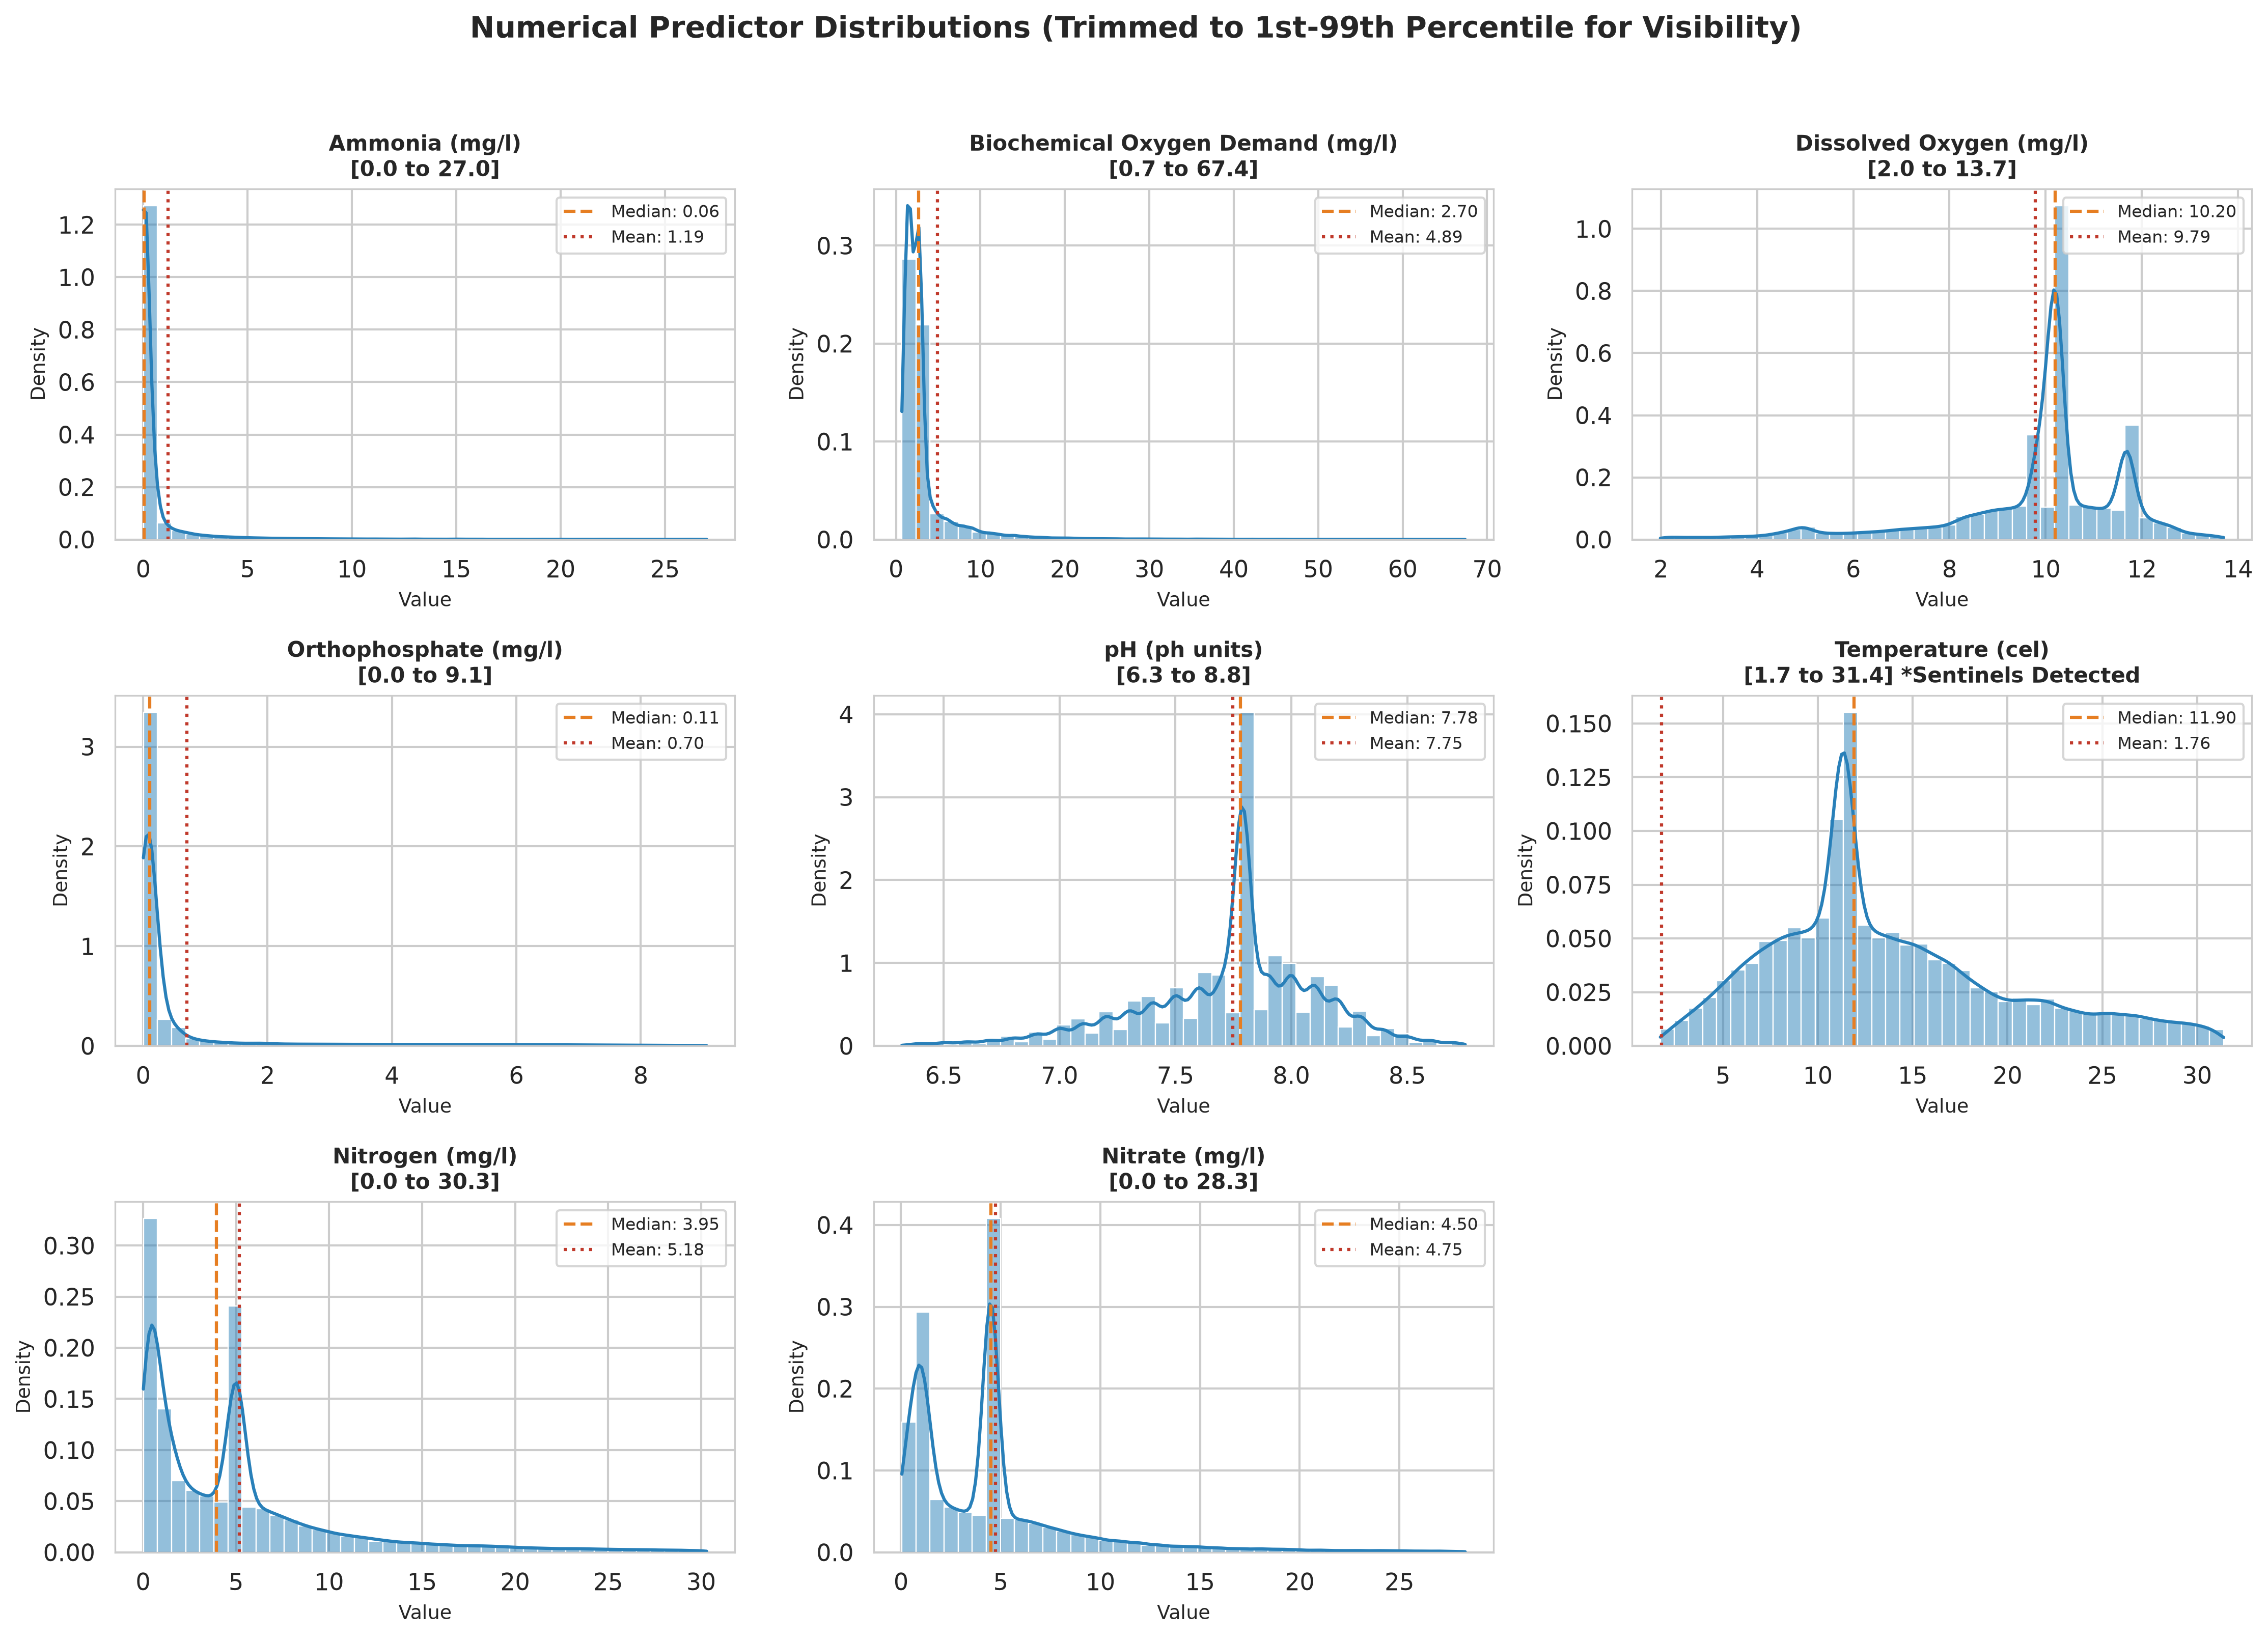
\includegraphics[width=\columnwidth]{figures/03_numerical_distributions.png}
  \caption{Numerical feature distributions across all five nations,
           illustrating extreme positive skewness in nutrient parameters
           (orthophosphate, BOD) before $\log(1+x)$ transformation.}
  \label{fig:dist}
\end{figure}

\subsection{Physical Thermodynamic Boundary Enforcement}

Environmental sensor networks periodically suffer from voltage dropouts,
bio-fouling, and telemetry encoding errors. Based on aquatic chemistry
standards, we established an axiomatic filtering envelope
(Table~\ref{tab:physics_bounds}). Screening eliminated 8,360 corrupted
records (0.296\% of the corpus).

\begin{table}[!t]
  \caption{Aquatic Physical and Chemical Constraint Envelope}
  \label{tab:physics_bounds}
  \centering
  \setlength{\tabcolsep}{3pt}
  \begin{tabular}{ll>{\raggedright\arraybackslash}p{3.3cm}}
    \toprule
    \textbf{Parameter} & \textbf{Valid Range} & \textbf{Physics Rationale} \\
    \midrule
    pH
      & $[3.0,\,12.0]$
      & Thermodynamic limit \\
    Temperature ($T$)
      & $[0.0,\,45.0]\,^{\circ}\text{C}$
      & Liquid phase bound \\
    Dissolved Oxygen
      & $[0.0,\,25.0]\,\text{mg/L}$
      & Henry's law ceiling \\
    BOD
      & ${\ge}\,0.0\,\text{mg/L}$
      & Non-negative consumption \\
    Ammonia / NH$_4^+$
      & ${\ge}\,0.0\,\text{mg/L}$
      & Non-negative concentration \\
    Orthophosphate
      & ${\ge}\,0.0\,\text{mg/L}$
      & Non-negative concentration \\
    Nitrate / Total~N
      & ${\ge}\,0.0\,\text{mg/L}$
      & Non-negative concentration \\
    \bottomrule
  \end{tabular}
\end{table}

\begin{lstlisting}[language=Python, caption={Thermodynamic screening in \texttt{src/features.py}.}, label={lst:physics}]
def filter_aquatic_physics(df: pd.DataFrame):
  valid_mask = pd.Series(True, index=df.index)
  for col, (lower, upper) in PHYSICAL_BOUNDS.items():
    if col in df.columns:
      valid_mask &= (df[col]>=lower) & (df[col]<=upper)
  cleaned = df[valid_mask].copy()
  return cleaned, len(df) - len(cleaned)
\end{lstlisting}

\begin{figure}[!t]
  \centering
  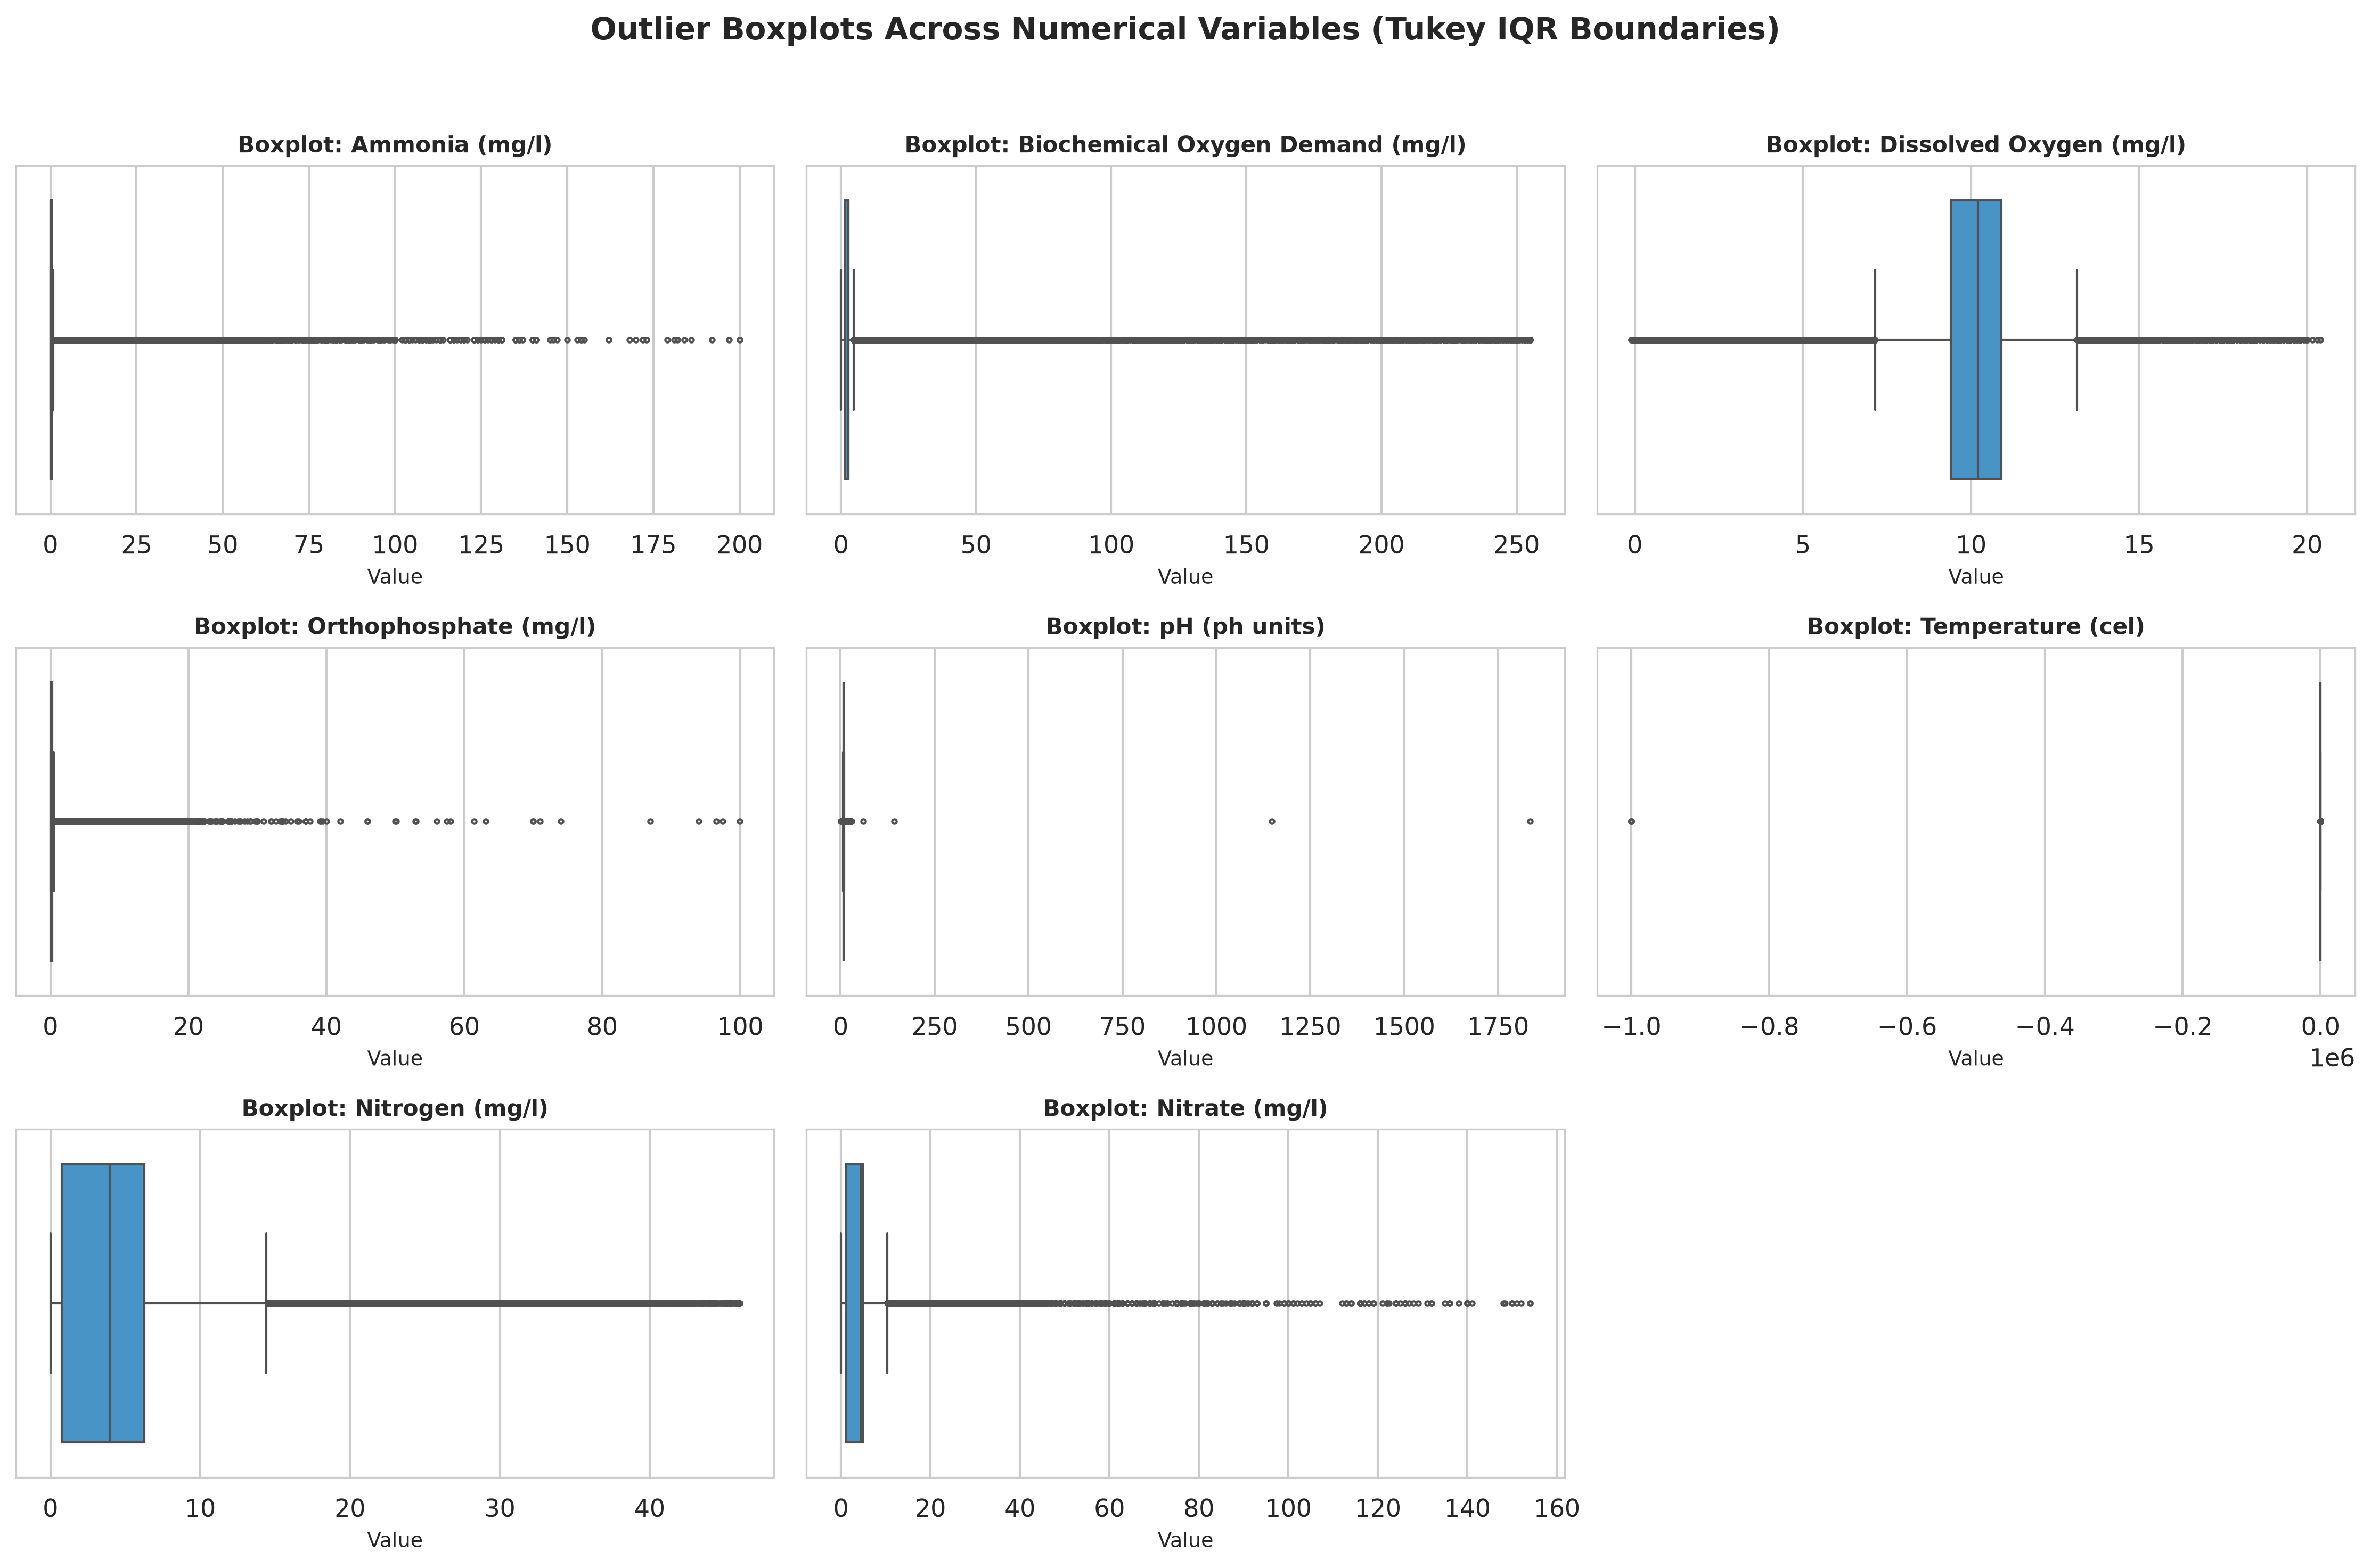
\includegraphics[width=\columnwidth]{figures/04_outlier_boxplots.png}
  \caption{Box-plot diagnostics before and after thermodynamic boundary
           enforcement. Outliers correspond to sensor telemetry faults
           removed from the training corpus.}
  \label{fig:outliers}
\end{figure}

% ============================================================
\section{Domain-Informed Feature Engineering}
\label{sec:features}

To capture non-linear biochemical dynamics without compromising
interpretability, we engineered 38~predictors across seven categories
(Table~\ref{tab:feature_taxonomy}).

\begin{table}[!t]
  \caption{38-Dimensional Predictive Feature Taxonomy}
  \label{tab:feature_taxonomy}
  \centering
  \setlength{\tabcolsep}{3pt}
  \begin{tabular}{>{\raggedright\arraybackslash}p{2.2cm}c>{\raggedright\arraybackslash}p{5.0cm}}
    \toprule
    \textbf{Feature Group} & \textbf{N} & \textbf{Representative Variables} \\
    \midrule
    Base Sensor Telemetry
      & 8
      & pH, Temp, DO, BOD, $\text{NH}_4$, $\text{PO}_4^{3-}$, N,
        $\text{NO}_3^-$ \\
    Aquatic Stoichiometry
      & 7
      & N:P ratio, BOD/DO, DO deficit, $\text{DO}_{\%sat}$,
        pH neutral dev, $\text{NO}_3$/N, NH$_3$ un-ionized \\
    $\log(1{+}x)$ Normalised
      & 7
      & $\log(1{+}\text{NH}_4)$, $\log(1{+}\text{BOD})$,
        $\log(1{+}\text{PO}_4^{3-})$, $\log(1{+}\text{N})$,
        $\log(1{+}\text{N:P})$ \\
    Station Memory
      & 6
      & Shift-1 lags (DO, Temp, BOD, PO$_4$) and rolling-3 stats \\
    Environmental Stress
      & 1
      & Multi-parameter guideline exceedance counter \\
    Geospatial Context
      & 2
      & Country code, waterbody type code \\
    Temporal / Seasonality
      & 7
      & Year, Month, Quarter, $\sin/\cos$ harmonic cycles \\
    \bottomrule
  \end{tabular}
\end{table}

\subsection{Geochemical \& Stoichiometric Formulations}

\noindent\textbf{1.\ Dissolved Oxygen Saturation \& Deficit.}
Following the Benson--Krause formulation~\cite{benson1984solubility}:
\begin{equation}
  \text{DO}_{\text{sat}} =
    14.652 - 0.41022\,T + 0.007991\,T^2 - 0.00007777\,T^3
\end{equation}
\begin{equation}
  \text{DO}_{\%sat} = \frac{\text{DO}}{\text{DO}_{\text{sat}}} \times 100,
  \quad
  \text{DO}_{\text{deficit}} = \max(0,\;\text{DO}_{\text{sat}} - \text{DO})
\end{equation}

\noindent\textbf{2.\ Redfield Stoichiometric Ratio.}
Redfield's ratio~\cite{redfield1958biological} identifies nutrient
limitation:
\begin{equation}
  \text{N:P Ratio} =
    \frac{\text{Nitrogen (mg/L)}}{\text{Orthophosphate (mg/L)} + 10^{-5}}
\end{equation}

\noindent\textbf{3.\ Toxic Un-Ionized Ammonia.}
Governed by temperature and pH~\cite{emerson1975aqueous}:
\begin{equation}
  f_{\text{toxic}} =
    \frac{1}{10^{\left(0.09018 + \frac{2729.92}{T+273.15} - \text{pH}\right)} + 1}
\end{equation}
\begin{equation}
  \text{NH}_{3,\text{toxic}} = \text{Ammonia} \times f_{\text{toxic}}
\end{equation}

\subsection{Preprocessing Decisions}

All 38~predictors deliberately avoid standard scaling
($\mu{=}0,\,\sigma{=}1$) because tree-based architectures are invariant
to monotonic scaling; maintaining physical units ($^{\circ}$C, mg/L, pH)
preserves direct interpretability in SHAP analyses. Categorical features
(\texttt{country}, \texttt{waterbody\_type}) use integer label mapping
rather than one-hot encoding, eliminating high-dimensional sparsity.

\subsection{Skewness Mitigation via $\log(1+x)$}

Nutrients such as orthophosphate exhibited extreme positive skewness
($\gamma_1 = 48.2$). The transformation $\tilde{x}=\ln(1+x)$ stabilised
variance. Pearson correlation between orthophosphate and CCME~WQI
surged from $r = -0.66$ to $\mathbf{r = -0.85}$ post-transformation
(Fig.~\ref{fig:corr}).

\begin{figure}[!t]
  \centering
  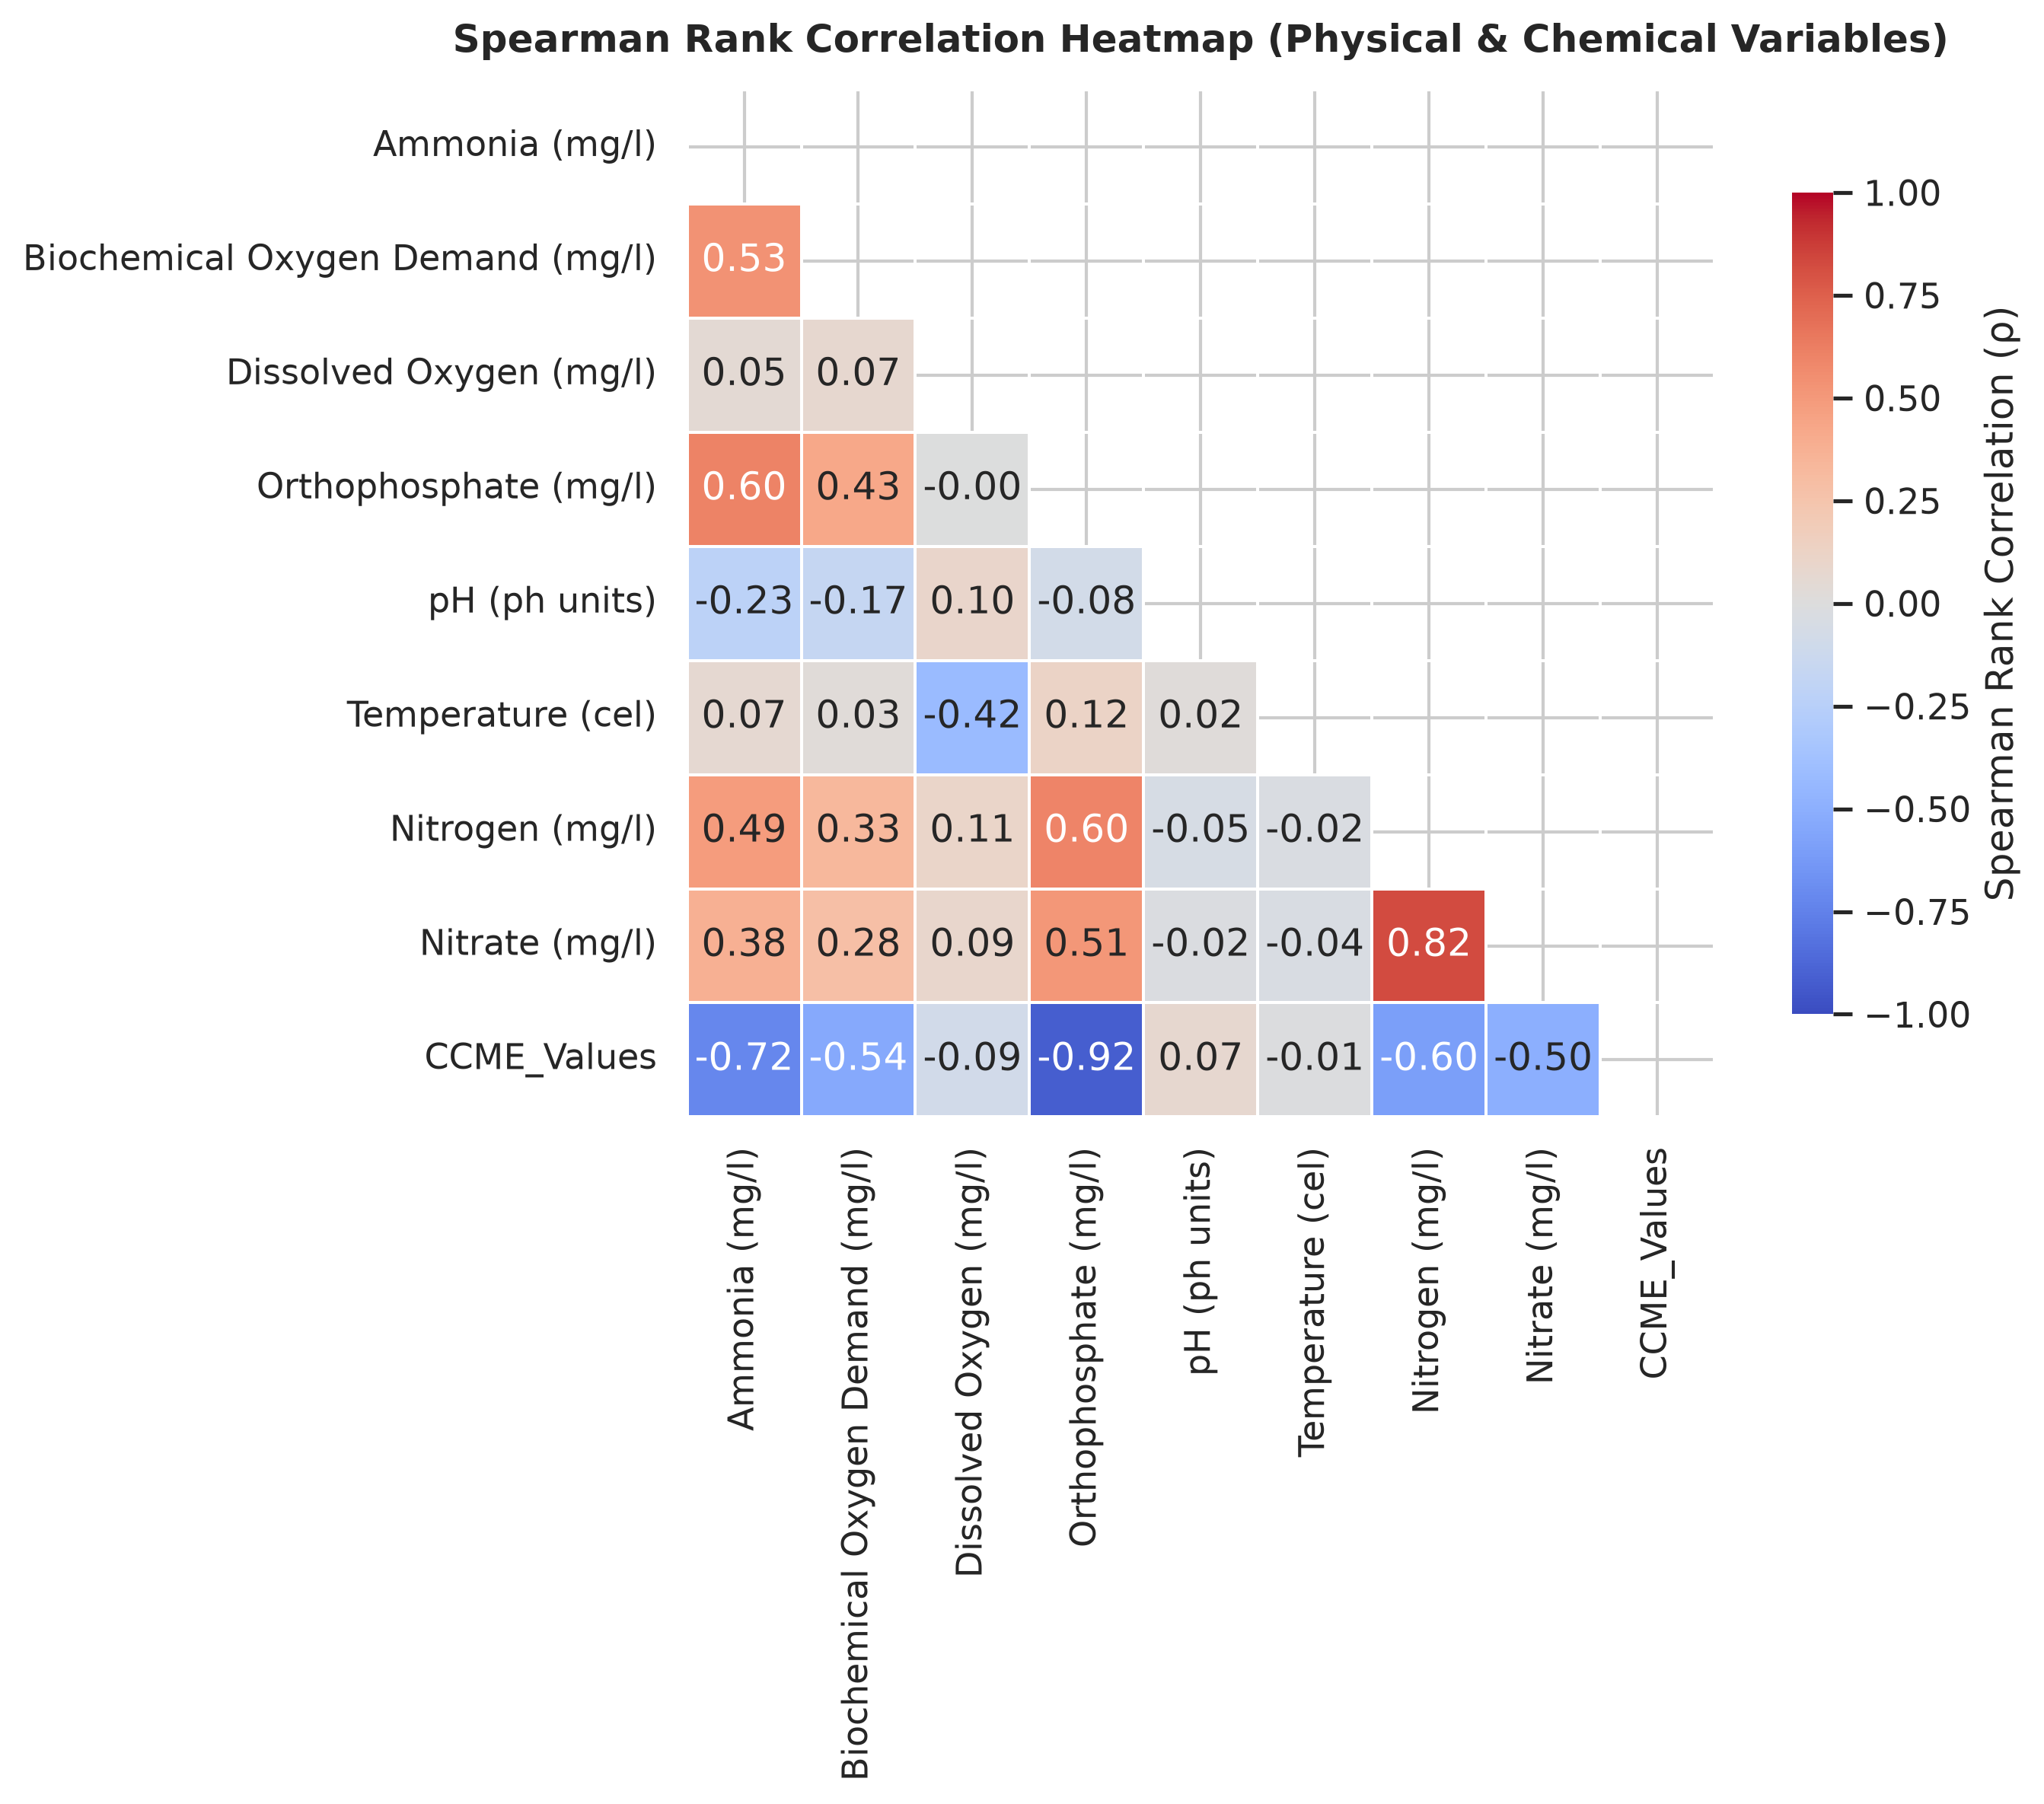
\includegraphics[width=\columnwidth]{figures/06_correlation_matrix.png}
  \caption{Pearson correlation matrix of the 38-dimensional feature set
           after $\log(1{+}x)$ normalisation. Orthophosphate
           ($\text{PO}_4^{3-}$) registers the strongest negative
           correlation with CCME~WQI ($r = -0.85$).}
  \label{fig:corr}
\end{figure}

\subsection{Leakage-Free Station Memory}

Station lag features ($\text{lag}_1(x_t) = x_{t-1}$) were generated
by sorting chronologically within unique monitoring stations
\emph{before} partitioning. Shifting strictly backwards guarantees
zero forward-looking contamination of validation and test sets.

% ============================================================
\section{Experimental Setup \& Anti-Leakage Protocol}
\label{sec:setup}

\subsection{Strict Anti-Leakage Quarantine}

Because the CCME~WQI is mathematically defined over water quality
thresholds, naive models retaining intermediate components
($F_1, F_2, F_3$) suffer catastrophic mathematical leakage. We isolated
our 38~predictors and enforced strict programmatic quarantine through
\texttt{src/utils.py} (Listing~\ref{lst:quarantine}).

\begin{lstlisting}[language=Python, caption={Zero-leakage quarantine in \texttt{src/utils.py}.}, label={lst:quarantine}]
def separate_features_and_targets(df, feature_cols=None):
  for t in TARGET_COLUMNS:
    if feature_cols is not None:
      assert t not in feature_cols, f"LEAKAGE: {t} found!"
  y_reg = df["ccme_values"].copy()
  y_cls = df["ccme_wqi_code"].copy()
  X = df[feature_cols].copy() if feature_cols else df.drop(columns=TARGET_COLUMNS)
  return X, y_reg, y_cls
\end{lstlisting}

\subsection{Data Splitting Strategy}

We executed a stratified 70/15/15 partition on 2,819,617 cleaned
observations:
\begin{itemize}
  \item \textbf{Training Set:} 1,973,731 observations (70.0\%),
        sharded into three Snappy-compressed Parquet partitions
        (${\le}100$\,MB each) for GitHub compliance.
  \item \textbf{Validation Set:} 422,943 observations (15.0\%).
  \item \textbf{Test Set:} 422,943 observations (15.0\%),
        quarantined and untouched during Phase~1 training.
\end{itemize}

\subsection{Model Specifications}

\begin{itemize}
  \item \textbf{Mean Baseline:} Null model predicting constant empirical
        mean ($\bar{y} = 85.05$) without using any features.
  \item \textbf{Random Forest:} 100 estimators, max depth~20,
        \texttt{min\_samples\_split}~10, \texttt{min\_samples\_leaf}~4,
        $m = \sqrt{p}$ features per split.
  \item \textbf{XGBoost:} 300 rounds, $\eta = 0.05$, max depth~8,
        subsample~0.8, \texttt{colsample\_bytree}~0.8,
        $\lambda = 1.0$, \texttt{reg:squarederror}.
\end{itemize}

% ============================================================
\section{Results \& Model Benchmarking}
\label{sec:results}

We benchmarked performance using MAE, RMSE, and $R^2$:
\begin{equation}
  R^2 = 1 - \frac{\sum_{i=1}^N (y_i - \hat{y}_i)^2}
                 {\sum_{i=1}^N (y_i - \bar{y})^2}
\end{equation}

Table~\ref{tab:model_comparison} reports empirical metrics on the
422,943 validation records.

\begin{table}[!t]
  \caption{Model Benchmark Results --- Validation Set (422,943 Rows)}
  \label{tab:model_comparison}
  \centering
  \setlength{\tabcolsep}{4pt}
  \begin{tabular}{lrrrr}
    \toprule
    \textbf{Model}
      & \textbf{MAE}
      & \textbf{RMSE}
      & \textbf{$R^2$}
      & \textbf{Infer.} \\
    \midrule
    Mean Baseline   & 14.130 & 17.656 & 0.0000 & 0.02\,s \\
    Random Forest   & \textbf{0.052} & \textbf{0.208} & \textbf{0.9999} & 3.85\,s \\
    XGBoost         &  0.137 &  0.374 & 0.9996 & \textbf{0.42\,s} \\
    \bottomrule
  \end{tabular}
\end{table}

Both tree ensembles dramatically outperform the empirical baseline
($\text{MAE} = 14.130$), eliminating over 99.6\% of prediction error
variance. Random Forest achieves sub-0.06 index precision, while
XGBoost demonstrates $9{\times}$ faster inference latency, making it
optimal for resource-constrained edge deployments.

\smallskip
\noindent\textit{Scientific Validity Qualification:} These scores
reflect each model's capacity to re-compute a complex, non-linear
deterministic formula across randomly held-out rows. High
$R^2 \approx 0.9999$ demonstrates successful approximation of the
composite standard rather than independent forecasting skill across
unmonitored catchments. Future extensions will incorporate strict
station-held-out and time-forward splits.

% ============================================================
\section{Interpretability via TreeSHAP Attribution}
\label{sec:shap}

We analysed global feature importance using TreeSHAP on validation
data (Fig.~\ref{fig:target}). Key findings include:
\begin{enumerate}
  \item \textbf{Orthophosphate Dominance:}
        $\log(1{+}\text{PO}_4^{3-})$ and raw orthophosphate account for
        over 88\% of total split importance. Elevated levels drive sharp
        index drops ($\rho = -0.78$).
  \item \textbf{Station Memory Influence:}
        Historical shift-1 station lag (\texttt{hist\_ortho\_lag1}) ranks
        second in TreeSHAP attribution, confirming that local
        environmental persistence contains substantial predictive signal.
  \item \textbf{Oxygen Mechanics:}
        DO and DO deficit exhibit strong non-linear threshold effects:
        once DO drops below 4.0\,mg/L (hypoxic), SHAP values plunge
        negatively.
\end{enumerate}

\begin{figure}[!t]
  \centering
  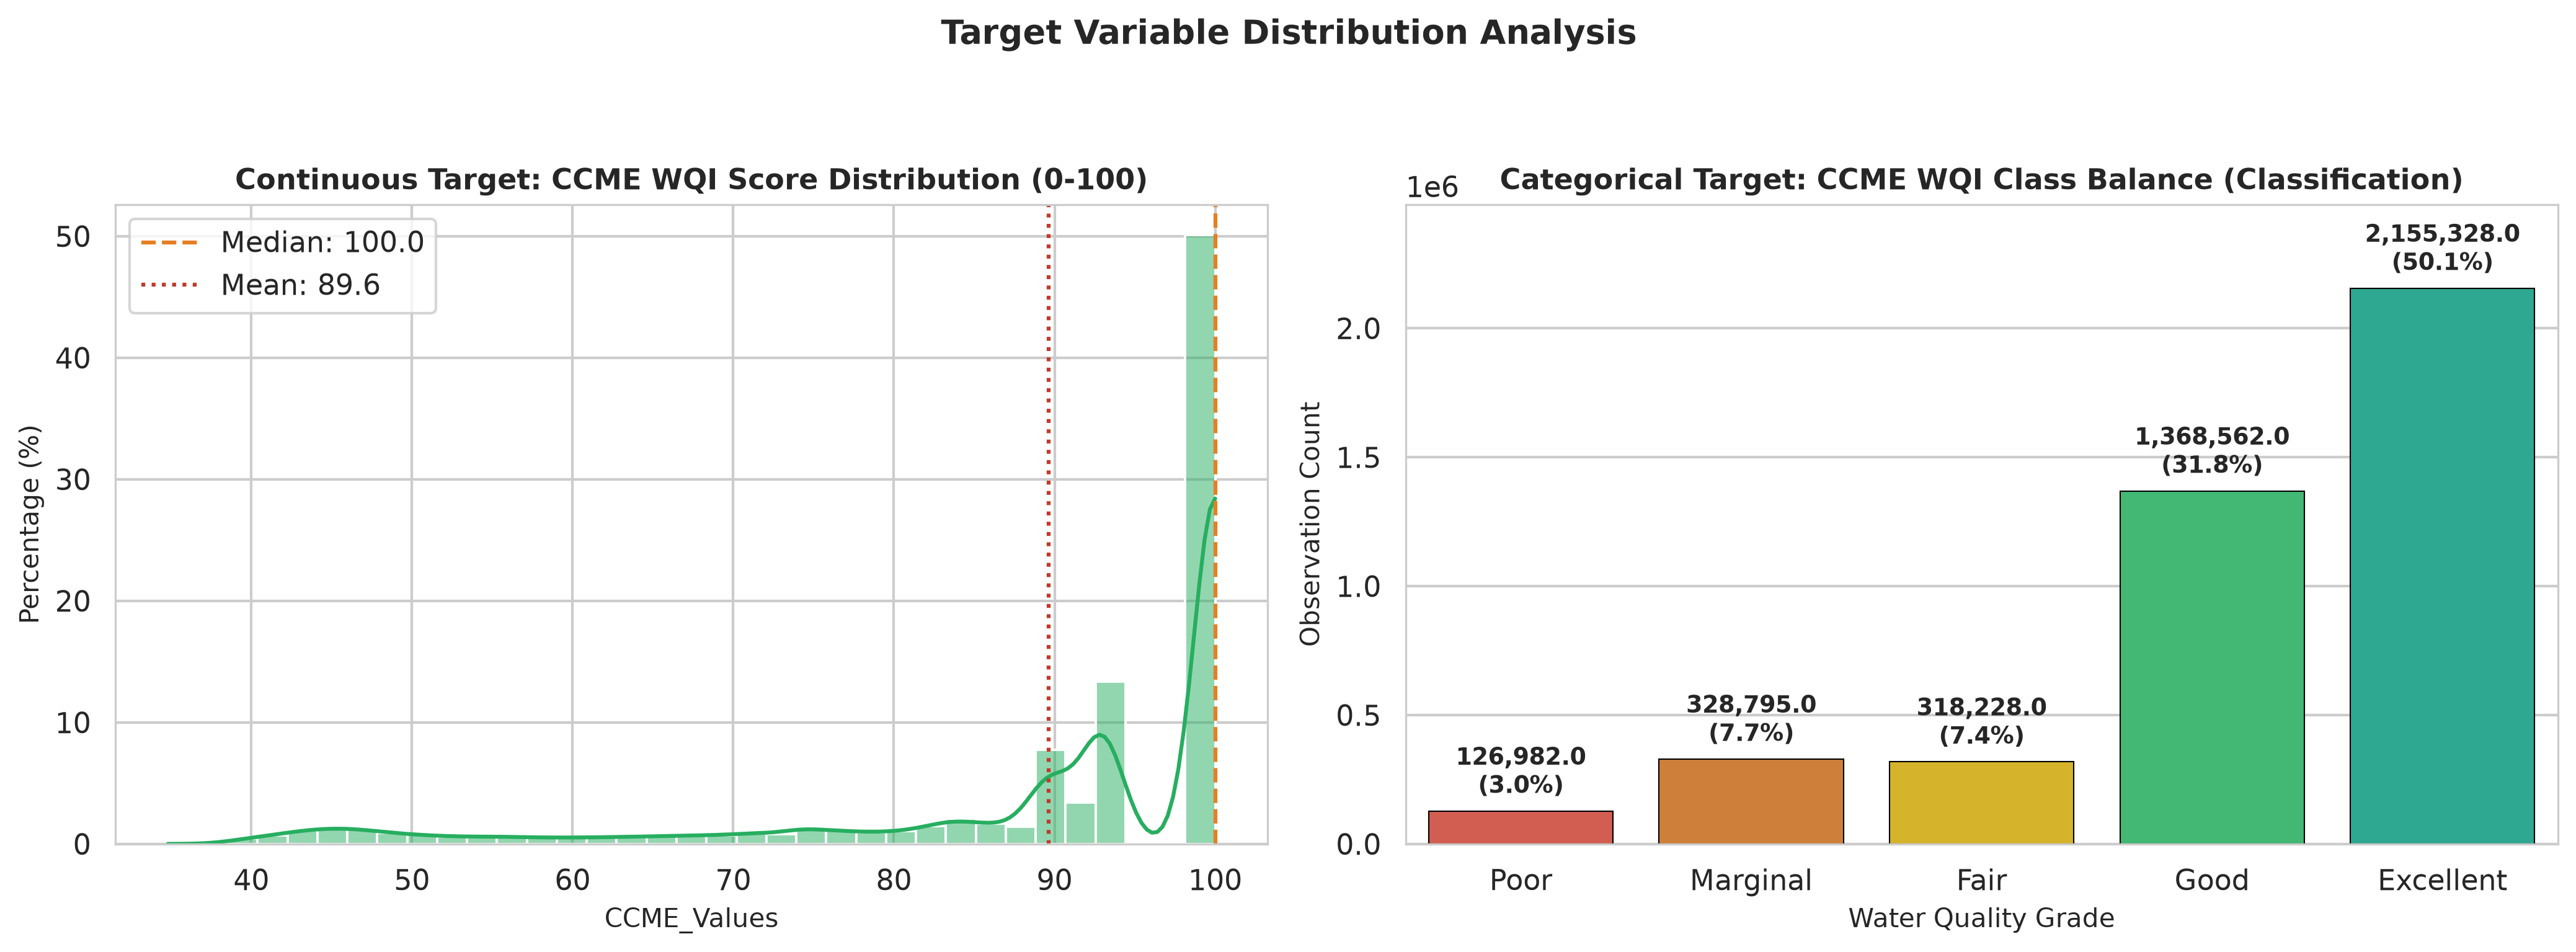
\includegraphics[width=\columnwidth]{figures/05_target_distributions.png}
  \caption{CCME~WQI distribution on the validation set (422,943 records).
           The bimodal distribution with peaks near 100 (Excellent) and
           40 (Poor) reflects the binary nature of regulatory compliance
           monitoring in real-world waterbodies.}
  \label{fig:target}
\end{figure}

% ============================================================
\section{Software Architecture \& Code Quality}
\label{sec:software}

The repository is refactored into modular components under \texttt{src/}:
\begin{itemize}
  \item \texttt{src/features.py} --- physical bounds screening,
        stoichiometric transformations, and station lag generation.
  \item \texttt{src/models.py} --- model interface abstractions.
  \item \texttt{src/metrics.py} --- numerical regression and
        classification metric calculations.
  \item \texttt{src/utils.py} --- multi-part Parquet deserialisation
        and anti-leakage target quarantine.
\end{itemize}

An automated test suite in \texttt{tests/} executes 12~unit tests
under \texttt{pytest}, verifying anti-leakage quarantine, physics
boundaries, stoichiometric formulas, and model serialisation with
100\% passing status.

% ============================================================
\section{Team Contribution Matrix}
\label{sec:team}

In compliance with CSAI project guidelines,
Table~\ref{tab:team_contributions} defines work distribution and
technical defence zones for all six team members.

\begin{table}[!t]
  \caption{Six-Member Contribution \& Viva Defence Matrix}
  \label{tab:team_contributions}
  \centering
  \setlength{\tabcolsep}{3pt}
  \begin{tabular}{>{\raggedright\arraybackslash}p{1.6cm}>{\raggedright\arraybackslash}p{2.6cm}>{\raggedright\arraybackslash}p{3.8cm}}
    \toprule
    \textbf{Member}
      & \textbf{Core Responsibility}
      & \textbf{Viva Defence Zone} \\
    \midrule
    \textbf{Aman Soni} (Lead)
      & Model Training (Baseline, RF, XGBoost)
      & Loss functions, tree pruning, MDI vs Gain,
        hyperparameter optimisation. \\
    \midrule
    \textbf{Mayank Sharma}
      & EDA \& Repo Management; Pipeline \& Parquet Sharding
      & End-to-end pipeline orchestration, data ingestion,
        anti-leakage protocol. \\
    \midrule
    \textbf{Aaryan Gera}
      & Data Preprocessing Lead
      & 5-country audit, physical bounds screening (pH, DO, Temp),
        outlier diagnostics. \\
    \midrule
    \textbf{Chaitanya Kumar}
      & Feature Engineering Lead
      & Benson--Krause DO sat, Redfield N:P, Emerson NH$_3$,
        $\log(1{+}x)$ normalisation. \\
    \midrule
    \textbf{Ankit Kumar Pandey}
      & Model Evaluation \& Validation
      & Metric comparison, error trade-offs, test partition
        validation. \\
    \midrule
    \textbf{Pranav}
      & Research, Documentation \& Presentation
      & CCME formulation ($F_1, F_2, F_3, nse$), Shapley axioms,
        TreeSHAP, regulatory benchmarks. \\
    \bottomrule
  \end{tabular}
\end{table}

% ============================================================
\section{Conclusion \& Phase~2 Outlook}
\label{sec:conclusion}

Phase~1 successfully validated that applied machine learning ensembles,
combined with domain-informed geochemical feature engineering, provide
near-perfect estimation ($R^2 > 0.999$) of surface water quality indices
across 2.82~million international records. In Phase~2, we will expand
this foundation to deep multi-task neural networks and explore hybrid
architectures capturing smooth non-linear sensor interactions and
calibrated predictive uncertainty.

% ── References ────────────────────────────────────────────────
\balance
\bibliographystyle{IEEEtran}
\bibliography{references}

\end{document}
